
\cleardoublepage
\chapter{Lernexperimente und Ergebnisse}\label{ch:TrainingsAndResults}

Dieses Kapitel beschäftigt sich mit dem Erlernen autonomer Fahrverhaltensweisen.
Zunächst werden die durchgeführten Trainingsläufe vorgestellt. Daraufhin folgt
eine Evaluation der daraus resultierenden Agenten anhand von Unfallmetriken.
Anschließend werden die Ergebnisse interpretiert und mit den Ergebnissen anderer
Ansätze verglichen. Zum Schluss wird noch auf die Minimierung der Trainingszeiten
durch eine Verbesserung der Sample Efficiency anhand einer Hyperparameteroptimierung
und der Anwendung von Modellbasiertem Lernen eingegangen.


\section{Durchführung der Trainingsläufe}

Im Laufe dieser wissenschaftlichen Arbeit werden eine Vielzahl an Trainingsläufen
durchgeführt. Die erfolgreichsten Agenten sind in Tabelle \ref{tab:TrainingRuns} zu sehen.
Außerdem stehen die Modelle und Videos des beobachteten Fahrverhaltens im Appendix zur
Verfügung. Im Folgenden werden die Versuche beschrieben und die vorgenommenen Adaptionen
an den Trainingsbedingungen begründet. Experiment 01 bezieht sich auf den Ansatz
der ursprünglichen Umsetzung von \emph{RobotSF} wie in \cite{machines11020268} und
dient als Grundlinie. Alle weiteren Experimente verwenden die Trainingsumgebungen
aus Abschnitt \ref{sec:TrainingApproach}.\\

\begin{table}[h]
  \centering
\begin{tabular}{ |p{1.5cm}||c|c|c|c|c|c|c|c| }
 \hline
 Training & Karte & Reward & Verkehr & Kinematik & Aktionen & $\Delta t$ & FE & PRF \\
 \hline \hline
 Exp. 01 & orig. & komplex & mittel    & Diff. Drive & wenig & 1 & nein & ja   \\ \hline
 Exp. 02 & klein & einfach & wenig     & Diff. Drive & wenig & 1 & nein & nein \\ \hline
 Exp. 03 & klein & einfach & viel      & Diff. Drive & wenig & 1 & nein & nein \\ \hline
 Exp. 04 & klein & einfach & viel      & Diff. Drive & wenig & 1 & nein & ja   \\ \hline
 Exp. 05 & klein & einfach & sehr viel & Diff. Drive & wenig & 1 & nein & ja   \\ \hline
 Exp. 06 & groß  & einfach & mittel    & Bicycle     & viel  & 3 & ja   & ja   \\ \hline
 Exp. 07 & groß  & einfach & mittel    & Bicycle     & viel  & 3 & ja   & ja   \\ \hline
 Exp. 08 & groß  & einfach & mittel    & Bicycle     & viel  & 3 & ja   & ja   \\
 \hline
\end{tabular}
\caption{Auflistung der Experimente und verwendeter Parameter}
\label{tab:TrainingRuns}
\end{table}

Zunächst liegt der Fokus bis einschließlich Experiment 05 auf einem Fahrzeug mit
Differential Drive Kinematik. Das Kartenmaterial besteht aus einigen miteinander verbundenen
Häuserblocks nahe des Universitätsgeländes, in deren Innenhöfen künstliche Fußgängerzonen
angelegt werden, um belebte Plätze zu simulieren. Das Fahrzeug startet in der Mitte
der Karte und folgt Routen in alle Himmelsrichtungen, die bewusst durch mindestens
eine Menschenmenge verlaufen. Durch die Wahl eines Zielradius von 1 Meter wird erzwungen,
dass der Fahragent lernt, sicher in die Menschenmenge einzutauchen und wieder herauszufahren.
Die \emph{Ped-Robot Force} (PRF) ist hierbei zunächst deaktiviert, sodass die Fußgänger
das Fahrzeug nicht wahrnehmen und demnach auch nicht ihrerseits ausweichen können.
Zudem liefert der LiDAR-Sensor nur die Entfernungen eines Zeitschritts (Standbild),
woraus für den Agent keine Fußgängerdynamiken ableitbar sind.
Des weiteren verfügt das Neuronale Netz des Agenten über keinen Feature Extractor (FE),
sondern verarbeitet flache, konkatenierte Feature-Vektoren aller Sensoren.
Die Fußgängerdichte wird während des Trainings auf 0.01 Fußgänger pro $m^2$
eingestellt, was einer relativ lückenhaften Menschenmenge entspricht und im Laufe der
Versuchsreihe hin zu moderaten Menschenmassen mit Dichte 0.04 erhöht. Anschließend
wird das Fahrverhalten der trainierten Agenten jeweils im Live Debugging begutachtet,
wobei schrittweise die Fußgängerdichte von 0.01 Fußgänger pro $m^2$ auf 0.08 angehoben wird.\\

Es kann bei den zugehörigen Experimenten 02 und 03 beobachtet werden, dass der Fahragent
erwartungsgemäß eine Strategie erlernt, die im fußgängerfreien Bereich geradlinig zum Ziel
fährt und beim Eintauchen in Menschenmengen ebenfalls zielstrebig eine Lücke findet,
um den jeweiligen Wegpunkt zu erreichen. Bei höheren Fußgängerdichten wird anstatt des
schnellen Eintauchens in die Menschenmenge ein abwartendes Verhalten beobachtet, wobei
der Agent so lange neben der Menge stehen bleibt, bis sich eine befahrbare Lücke öffnet.
Die gelernten Verhaltensweisen erfüllen zwar die von der Trainingsumgebung gestellte
Aufgabe, sind jedoch für praktische Erprobungen eher ungeeignet, da oftmals Situationen
vorliegen, bei denen kein Fortschritt zu erzielen ist, wenn nur außerhalb der
Menschenmenge gewartet wird.\\

Um praxistauglichere Verhaltensweisen zu erhalten, wird eine weitere Versuchsreihe
anhand der Experimente 04 und 05 mit moderaten bis hohen Fußgängerdichten und aktivierter
\emph{Ped-Robot Force} durchgeführt, sodass die Fußgänger nun das Fahrzeug sehen können
und eigenständig ausweichen. Die Kraft wird so gewichtet, dass ein stehendes Fahrzeug
relativ eng von den Fußgängern umlaufen wird. Dadurch muss der Agent keine Zusammenstöße
befürchten, ist aber zugleich zum Abwarten gezwungen, bis die Passage frei ist. Bei einem
entsprechend trainierten Agent wird ein Fahrverhalten beobachtet, bei dem das Fahrzeug
frontal in die Menschenmenge eintaucht und sich langsam je nach Freiraum vor dem
Fahrzeug vorwärts zum Wegpunkt bewegt. Wie in Abbildung \ref{fig:DiveIntoCrowd} zu
sehen ist, bleibt das Fahrzeug stehen und lässt die Fußgänger passieren, solange
es komplett von Fußgängern umgeben ist und wartet ab, bis erneut Fortschritte
zu erzielen sind. Diese Verhaltensweise liefert zufriedenstellende Ergebnisse,
jedoch lenkt der Agent nach dem Erreichen von Wegpunkten teilweise abrupt, da ihm
die Peilung des nächsten Wegpunkts nicht bekannt ist und er zudem durch eine niedrige
Aktionsfrequenz von nur 2.5 Aktionen pro Sekunde keine Möglichkeit für exaktere
Reaktionen hat.\\

\begin{figure}[h]
  \centering
  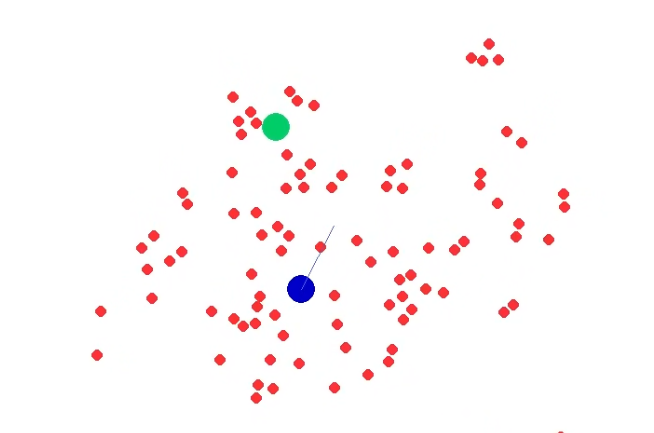
\includegraphics[width = 0.6\textwidth]{imgs/eintauchen_in_menschenmasse}
  \caption{Sicheres Durchqueren einer dichten Menschenmasse}
  \label{fig:DiveIntoCrowd}
\end{figure}

Um dynamischere Trajektorien fahren zu können, wird dem Agent eine zusätzliche
Zielpeilung des nächsten Wegpunkts bezüglich seiner aktuellen Orientierung
bereitgestellt. Zudem wird die Aktionsfrequenz auf 10 Aktionen pro Sekunde erhöht,
um eine exaktere Fahrweise zu ermöglichen. Der anschließende Trainingslauf bringt
jedoch keine wesentliche Verbesserung und wird deshalb verworfen. Es wird experimentell
nachgewiesen, dass die bei einer niedrigen Aktionsfrequenz trainierten Agenten in einer
Simulationsumgebung mit hoher Aktionsfrequenz gute Ergebnisse erzielen. Dies ist
vermutlich auf die sehr defensive Fahrweise der Agenten zurückzuführen, wofür nicht
so viele Aktionen pro Sekunde notwendig sind.\\

Da mit den bisherigen Trainingsläufen bereits sehr gute Verhaltensweisen in dichten
Menschenmengen erzielbar sind, wird nun eine größere Karte des Universitätscampus
als Trainingsumgebung verwendet, die Fußgängerrouten auf allen befahrenen Gehwegen und
einige Fußgängerzonen an Engstellen aufweist. Um die Erlernbarkeit der Steuerung eines
selbstfahrenden E-Scooters zu demonstrieren, wird eine zusätzliche Fahrzeugkinematik
anhand des Fahrradmodells erprobt. Zur Modellierung von Fußgängerdynamiken stehen
dem Agent die Sensordaten der letzten 3 Simulationsschritte zur Verfügung, welche mit
einem Feature Extractor vorverarbeitet werden.\\

Die aus den folgenden Experimente 06, 07 und 08 resultierenden Agenten sind durch die
neue Kinematik anhand des Fahrradmodells in der Lage, rückwärts zu fahren, wodurch
sich die erlernte Verhaltensweise stark ändert. Durch die zudem verbesserte Erkennung der
Fußgängerdynamiken können gefährlichere Fahrmanöver beobachtet werden, bei denen der
Agent auf einem Gehweg frontal auf einen entgegenkommenden Fußgänger zu fährt, im letzten
Moment stark rückwärts beschleunigt und dann eine ausweichende Kreisbahn einschlägt.
Eine entsprechende Verhaltensweise scheint für den echten Verkehr jedoch ungeeignet,
weshalb in der Fahrzeugkinematik das Rückwärtsfahren anschließend verboten wird.
Eine darauffolgende Auswertung ohne Rückwärtsfahren bestätigt die Annahme, dass der Agent
das Rückwärtsfahren aktiv in seinen Fahrmanövern einsetzt, da der Agent nun beim Ausweichen
rückwärts fahren möchte, aber nicht mehr kann und daraufhin mit dem Fußgänger kollidiert.\\

Weitere Experimente können aufgrund des beschränkten zeitlichen Rahmens dieser Arbeit
nicht mehr durchgeführt werden. Offene Fragen bleiben, wie gut ein Agent mit Differential
Drive Kinematik bzw. Fahrradmodell ohne Rückwärtsfahren in der großen Trainingsumgebung
des Universitätscampus lernt.


\section{Evaluation mittels Unfallmetriken}
Zur Auswertung der erlernten Fahragenten werden die in Abschnitt \ref{sec:EvalMetrics} definierten
Unfallmetriken herangezogen. Als Kartenmaterial dient der Campus der Universität Ausgburg.
Die Agenten steuern ein Fahrzeug mit denselben kinematischen Eigenschaften wie zur
Trainingszeit.\\

Um das erlernte Verhalten bereits während des Trainings
beurteilen zu können, werden entsprechende Metriken zudem auch mittels gleitendem Durchschnitt
über die letzten 10 gefahrenen Routen pro Simulationsumgebung erhoben. Wie in Abbildung
\ref{fig:TypicalCollRates} dargestellt zeigt sich allgemein, dass die Agenten zu Beginn eines
Trainingslaufs zunächst lernen, Kollisionen zu vermeiden, jedoch oftmals den anzusteuernden
Wegpunkt nicht erreichen, was sich in einer erhöhten \emph{Timeout Rate} bzw. Episodendauer äußert.
Anschließend erfolgt die Erprobung von Fahrmanövern, wobei die dafür benötigte, simulierte Zeit
minimiert wird, was durch eine langsam sinkende, durchschnittliche Episodendauer messbar ist.
Da der Agent nun riskantere Fahrmanöver auswählt, erhöhen sich in der Regel die Kollisionsraten.
Stationären Hindernissen kann leicht ausgewichen werden, weshalb es hauptsächlich zu Kollisionen
mit Fußgängern kommt. Gegen Ende des Trainings lernt der Agent schließlich, die Bewegung der
Fußgänger zu interpretieren und ihnen effektiv auszuweichen.\\

\begin{figure}[h]
  \centering
  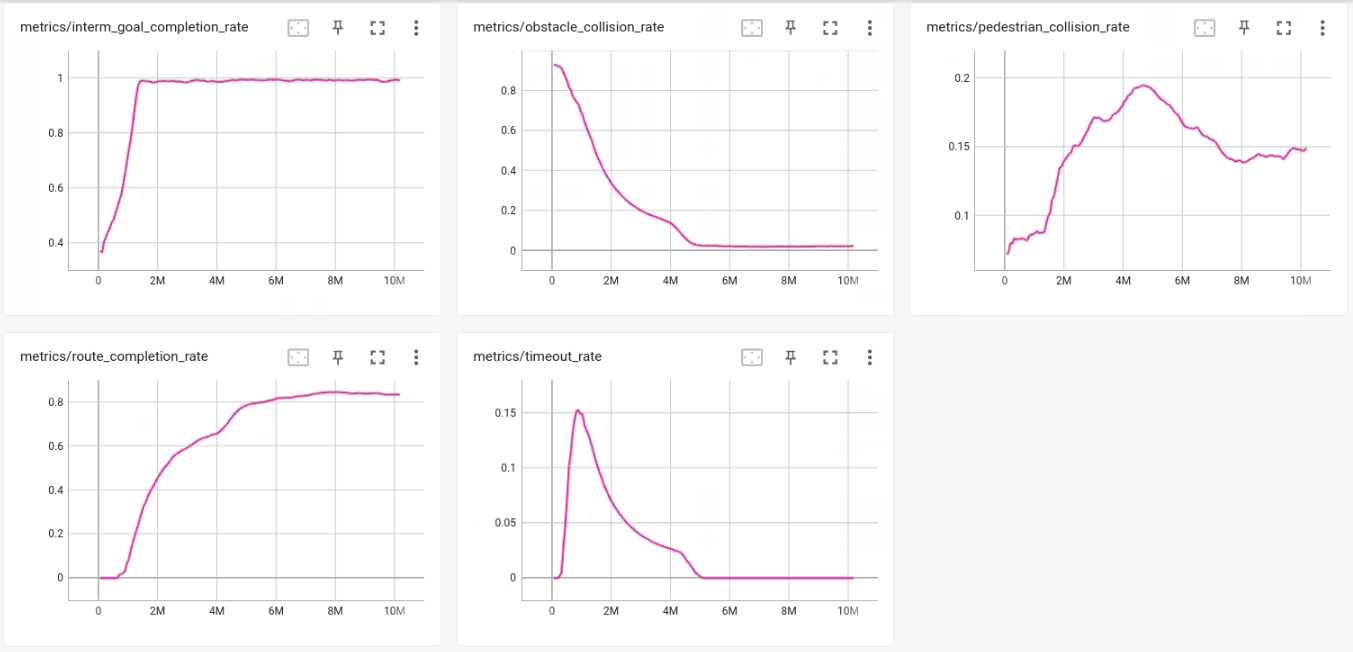
\includegraphics[width = 1.0\textwidth]{imgs/unfallraten_typisches_beispiel}
  \caption{Typischer Verlauf der Unfallmetriken während des Trainings. Zu sehen
  sind zeilenweise von rechts nach links die Komplettierungsrate von Wegpunkt
  zu Wegpunkt, die Kollisionsraten mit Fußgängern bzw. Hindernissen, die Rate
  komplettierter Routen und die Timeout-Rate. Auf x- und y-Achse sind jeweils die Zeit
  und die Rate zwischen 0 und 1 aufgetragen.}
  \label{fig:TypicalCollRates}
\end{figure}

Aufgrund der Stochastizität der erlernten Strategien unterliegen die Unfallmetriken
starken Schwankungen. Es genügen oftmals schon wenige, fehlerhafte Vorhersagen,
um einen Unfall herbeizuführen, der bei einer deterministischen Schätzung nicht
geschehen wäre. Daher werden zur Evaluation immer die geschätzten Mittelwerte für die
Aktuatoren statt der während des Trainings üblichen, normalverteilten Schätzungen
verwendet. Aufgrund der Notwendigkeit, die für die Modellaktualisierung benötigten
Trainingsdaten mit einer stochastischen Strategie zu sammeln, haben zur Trainingszeit
erhobene Unfallmetriken nur eine geringe Aussagekraft und dienen lediglich als grobe
Anhaltspunkte. Die folgenden Ergebnisse werden deshalb mit deterministisch
vorhergesagten Aktionen austrainierter Agenten ausgewertet. Je Auswertung fährt der
Agent 100 Routen, sodass die resultierenden Ergebnisse auf 1\% genau sind. Insbesondere
für die Bereiche $[0.00, 0.01]$ und $[0.99, 1.00]$ besteht daher keine Aussagekraft.
Dies stellt jedoch kein Problem dar, da die zu vergleichenden Ergebnisse ohnehin
keine entsprechende Qualität aufweisen.\\

Zur Evaluation werden alle erfolgreichen Trainingsläufe aus Tablelle \ref{tab:TrainingRuns}
betrachtet. Experiment 01 dient als Grundlinie für die ursprüngliche Umsetzung der
Trainingsumgebung durch Caruso et. al \cite{machines11020268} bezüglich Kartenmaterial
und Rewardstruktur.

\begin{table}[h]
\centering
\begin{tabular}{ |p{3cm}||c|c|c|c| }
 \hline
 Unfallmetrik vs. Trainingslauf & Completion & Obst. Coll. & Ped. Coll. & Timeout \\
 \hline \hline
 Experiment 01 & 0.08 & 0.00 & 0.00 & 0.92 \\ \hline
 Experiment 02 & 0.81 & 0.19 & 0.00 & 0.00 \\ \hline
 Experiment 03 & 0.05 & 0.00 & 0.00 & 0.95 \\ \hline
 Experiment 04 & 0.30 & 0.00 & 0.00 & 0.70 \\ \hline
 Experiment 05 & 0.14 & 0.00 & 0.00 & 0.86 \\ \hline
 Experiment 06 & 0.73 & 0.27 & 0.00 & 0.00 \\ \hline
 Experiment 07 & 1.00 & 0.00 & 0.00 & 0.00 \\ \hline
 Experiment 08 & 1.00 & 0.00 & 0.00 & 0.00 \\
 \hline
 \end{tabular}
 \caption{Auswertung der Unfallzahlen ohne Fußgänger}
 \label{tab:EvalNoPeds}
\end{table}

Wie in Tabelle \ref{tab:EvalNoPeds} zu sehen ist, wird zunächst zur Kontrolle eine Auswertung
ohne Fußgänger durchgeführt, um zu prüfen, ob die jeweilige Fahrsoftware statischen Hindernissen
ausweichen kann und die einfachere Aufgabe ohne bewegliche Hindernisse einwandfrei lösen kann.
Hier wäre eine Rate von 100\% zu erwarten, da die Problemstellung deutlich einfacher als mit
Fußgängern ist. Es zeigt sich aber, dass einige Agenten die Problemstellung nur unzureichend
lösen, was vielfältige Gründe haben kann. Beispielsweise
ist in der Live-Ansicht beobachtbar, dass die Agenten aus den Experimenten 02 bis 05 die Route
bis ans Ziel fahren, aber den letzten Wegpunkt meiden, weil sich dieser zu nah an einem Gebäude
befindet. Vermutlich ist ein entsprechendes Verhalten auf den Mangel an Engstellen
im Kartenmaterial zurückzuführen. Interessanterweise schneidet der mit einer komplexen
Rewardstruktur trainierte Agent in einer Umgebung ohne Fußgänger erstaunlich schlecht ab,
was nur schwer nachvollziehbar ist. Hingegen können die aus den Experimenten 07 und 08
resultierenden Agenten überzeugen, was vermutlich daran liegt, dass die Agenten
mit demselben Kartenmaterial trainiert wurden.\\

\begin{table}[h]
\centering
\begin{tabular}{ |p{3cm}||c|c|c|c| }
 \hline
 Unfallmetrik vs. Trainingslauf & Completion & Obst. Coll. & Ped. Coll. & Timeout \\
 \hline \hline
 Experiment 01 & 0.89 & 0.00 & 0.00 & 0.11 \\ \hline
 Experiment 02 & 0.59 & 0.13 & 0.28 & 0.00 \\ \hline
 Experiment 03 & 0.07 & 0.00 & 0.60 & 0.33 \\ \hline
 Experiment 04 & 0.38 & 0.06 & 0.02 & 0.54 \\ \hline
 Experiment 05 & 0.64 & 0.00 & 0.00 & 0.36 \\ \hline
 Experiment 06 & 0.18 & 0.25 & 0.57 & 0.00 \\ \hline
 Experiment 07 & 0.95 & 0.02 & 0.03 & 0.00 \\ \hline
 Experiment 08 & 0.93 & 0.01 & 0.06 & 0.00 \\
 \hline
\end{tabular}
\caption{Auswertung der Unfallzahlen mit Fußgängerdichte 0.02}
 \label{tab:EvalFewPeds}
\end{table}

In der zweiten Evaluation, deren Ergebnisse in Tabelle \ref{tab:EvalFewPeds} zu sehen sind,
werden die trainierten Agenten in einer Umgebung mit einer geringen Fußgängerdichte getestet.
Hierbei wird geprüft, ob die jeweilige Fahrsoftware vereinzelten, beweglichen Hindernissen
ausweichen kann und dabei nicht mit statischen Hindernissen Kollidiert. Es zeigt sich,
dass die Agenten mit kinematischem Fahrradmodell und einer verbesserten Sensorik besonders
gut abschneiden, da sie die Bewegungsdynamiken aus den Sensordaten extrahieren und somit
deren Bewegung einschätzen können, um adäquat auszuweichen. Hingegen weisen die Experimente
mit Differential Drive Kinematik und einer aus Standbildern bestehenden Sensorik deutlich
defensivere Verhaltensweisen auf, was auch im Live Debugging zu beobachten ist. Der Ansatz
mit alter Belohnungsstruktur und Kartenmaterial aus Experiment 01 schneidet gut ab,
was möglicherweise auf den Belohnungsterm zur Annäherungung an den nächsten Wegpunkt
zurückzuführen ist.\\

\begin{table}[h]
\centering
\begin{tabular}{ |p{3cm}||c|c|c|c| }
 \hline
 Unfallmetrik vs. Trainingslauf & Completion & Obst. Coll. & Ped. Coll. & Timeout \\
 \hline \hline
 Experiment 01 & 0.20 & 0.08 & 0.07 & 0.65 \\ \hline
 Experiment 02 & 0.16 & 0.11 & 0.73 & 0.00 \\ \hline
 Experiment 03 & 0.02 & 0.04 & 0.76 & 0.18 \\ \hline
 Experiment 04 & 0.59 & 0.07 & 0.11 & 0.23 \\ \hline
 Experiment 05 & 0.61 & 0.04 & 0.00 & 0.35 \\ \hline
 Experiment 06 & 0.01 & 0.20 & 0.79 & 0.00 \\ \hline
 Experiment 07 & 0.60 & 0.09 & 0.30 & 0.01 \\ \hline
 Experiment 08 & 0.51 & 0.13 & 0.35 & 0.01 \\
 \hline
\end{tabular}
\caption{Auswertung der Unfallzahlen mit Fußgängerdichte 0.08}
 \label{tab:EvalManyPeds}
\end{table}

In den letzten beiden Evaluationen, deren Ergebnisse in den Tabellen \ref{tab:EvalManyPeds}
und \ref{tab:EvalVeryCrowded} zu sehen sind, werden die trainierten Agenten in einer Umgebung
mit sehr dichtem Verkehr getestet. Hierbei steht die Unfallvermeidung, ohne Schäden an Personen,
Hindernissen und dem Fahrzeug zu verursachen im Vordergrund. Um die Aufgabe anspruchsvoller
zu gestalten, müssen die Agenten bewusst durch belebte Zonen hindurch fahren, was durch
entsprechend positionierte Wegpunkte erreicht wird. Die Schwierigkeit der Aufgabe besteht nun
darin, selbst bei dichtem Verkehr noch sicher Fortschritte erzielen zu können. Um die Aufgabe
überhaupt lösbar zu gestalten, weichen die Fußgänger dem Fahrzeug mittels \emph{Ped-Robot Force}
aus. Besonders hervorzuheben sind die Ergebnisse aus Experiment 05, wobei keine einzige
Kollision mit Fußgängern festzustellen ist. Der Agent kommt mit einer Ankunftsrate von
über 60\% am Routenziel an und wartet in fast allen weiteren Fällen ab. Die Ansätze
mit kinematischem Fahrradmodell und verbesserter Sensorik erreichen auch noch nennenswert
oft ihr Ziel, weisen jedoch eine offensive Fahrweise auf. Dies kann zum einen an der
Durchführung der Trainingsläufe bei weitaus geringerer Verkehrsdichte liegen.
Zum anderen ist auch denkbar, dass sich die Agenten zu sicher sind, die Dynamiken
der Fußgänger korrekt einschätzen zu können, was anschließend zu Unfällen führt.
Der mit komplexer Rewardstruktur trainierte Agent aus Experiment 01 kann nur schwer
Fortschritte erzielen, verursacht jedoch auch keine erhebliche Anzahl an Unfällen.

\begin{table}[h]
\centering
\begin{tabular}{ |p{3cm}||c|c|c|c| }
 \hline
 Unfallmetrik vs. Trainingslauf & Completion & Obst. Coll. & Ped. Coll. & Timeout \\
 \hline \hline
 Experiment 01 & 0.07 & 0.10 & 0.12 & 0.71 \\ \hline
 Experiment 02 & 0.10 & 0.18 & 0.72 & 0.00 \\ \hline
 Experiment 03 & 0.02 & 0.00 & 0.79 & 0.19 \\ \hline
 Experiment 04 & 0.39 & 0.10 & 0.20 & 0.31 \\ \hline
 Experiment 05 & 0.62 & 0.03 & 0.00 & 0.35 \\ \hline
 Experiment 06 & 0.00 & 0.17 & 0.83 & 0.00 \\ \hline
 Experiment 07 & 0.50 & 0.15 & 0.32 & 0.03 \\ \hline
 Experiment 08 & 0.33 & 0.14 & 0.52 & 0.01 \\
 \hline
\end{tabular}
\caption{Auswertung der Unfallzahlen mit Fußgängerdichte 0.10}
 \label{tab:EvalVeryCrowded}
\end{table}

\section{Vergleich der Ergebnisse}
Für einen fairen Vergleich werden die veröffentlichten Ergebnisse von Caruso et. al
\cite{machines11020268} herangezogen, da hier die meisten fachlichen und
konzeptionellen Überschneidungen bestehen und dieselben Unfallmetriken zur Auswertung
verwendet werden. Ihre Ergebnisse werden in Tabelle \ref{tab:EvalTriest}
zusammegefasst.\\

\begin{table}[h]
\centering
\begin{tabular}{ |p{3cm}||c|c|c|c| }
 \hline
 Unfallmetrik vs. Fußgängerdichte & Completion & Obst. Coll. & Ped. Coll. & Timeout \\
 \hline \hline
 0.00 / $m^2$ & 1.00 & 0.00 & 0.00 & 0.00 \\ \hline
 0.02 / $m^2$ & 0.87 & 0.00 & 0.13 & 0.00 \\ \hline
 0.08 / $m^2$ & 0.67 & 0.00 & 0.32 & 0.01 \\ \hline
 0.10 / $m^2$ & 0.52 & 0.01 & 0.47 & 0.00 \\ \hline
\end{tabular}
 \caption{Auswertung der Unfallzahlen von Caruso et. al \cite{machines11020268} mit A3C}
 \label{tab:EvalTriest}
\end{table}

Es zeigt sich, dass der Ansatz mit \emph{RobotSF} in seiner ursprünglichen Form zuverlässig
in Szenarien mit wenigen Fußgängern funktioniert und in etwa mit Experiment 07 vergleichbar
ist. Bei dichtem Verkehr weist die Fahrsoftware starke Schächen auf, da hohe Kollisionsraten
mit Fußgängern bestehen. Die defensive Strategie aus Experiment 05 erreicht ähnlich
gute Ankunftsraten, verursacht jedoch keine Kollisionen mit Fußgängern. Es kann also
von einer klaren Qualitätsverbesserung bei der Fahrsicherheit gesprochen werden.
Der Trainingsansatz, Agenten gezielt durch große Menschenmengen fahren zu lassen, scheint
vielversprechend. Ähnlich wie in Fan et. al \cite{fan2020distributed} könnte eine Kombination
einer defensiven und offensiven Fahrweise der Agenten aus Experiment 05 und 07 das Fahrverhalten
nochmals deutlich verbessern, indem bei wenig Verkehr die offensive und bei viel
Verkehr die defensive Fahrweise zum Einsatz kommt.\\

Da die Umsetzung einer Simulationsumgebung mit mehreren gleichzeitig agierenden Fahrzeugen
wie im Ansatz von \emph{Multi-Robot} zeitlich nicht mehr möglich war, ist ein Vergleich mit
Fan et. al \cite{fan2020distributed} nicht sinnvoll.


\section{Optimierung der Sample Efficiency}\label{sec:SampleEff}

Dieser Abschnitt befasst sich mit der Verbesserung der Trainingsdateneffizienz,
auch engl. Sample Efficiency genannt. Wie in vorherigen Abschnitten demonstriert wurde,
sind für qualitativ hochwertige Fahragenten keine rechenintensiven Neuronalen Netze
notwendig. Dementsprechend wenden Trainingsalgorithmen verhältnismäßig viel Zeit für
das Sammeln der Trainingsdaten auf. Ist eine hinreichende Performanz der Simulationsumgebung
hinsichtlich der inhärenten Berechnungskomplexität gegeben, muss das gewählte Lernverfahren
dahingehend optimiert werden, bereits gute Ergebnisse mit möglichst wenigen Trainingsdaten
zu erzielen. Die Durchführbarkeit von Lerntechniken des Bestärkenden Lernens in komplexen
Simulationsumgebungen hängt demnach stark von der Wahl eines geeigneten Lernverfahrens und
dessen Parametrisierung ab. In den folgenden Abschnitten wird daher untersucht,
wie die Trainingsdateneffizienz beim Erlernen von Fahrverhaltensweisen gesteigert werden kann.

\subsection{Optimierung der Lernparameter}
Wie bereits im Abschnitt über PPO \ref{sec:ppo} erläutert, kann die Trainingsdateneffizienz
erheblich durch die Wahl eines geeigneten Lernverfahrens gesteigert werden. Steht ein
geeigneter Lernalgorithmus fest, können dessen Parameter an die jeweilige Problemstellung
angepasst werden, um weitere Effizienzsteigerungen zu erreichen.\\

In diesem Zusammenhang stellt sich Effizienz als das Erlernen von Fahrqualität
pro Trainingszeit dar. Hierbei wird die Qualität durch die Rate unfallfrei gefahrener
Routen (\emph{Route Completion Rate}) und die Trainingszeit durch die simulierten
Trainingsschritte bemessen. Um diskrete Zeitpunkte bei der Erreichung einer gewissen
Qualität zu bestimmen, werden Qualitätsstufen in Schritten von jeweils 1\% definiert.
Die Anregung einer guten Qualität soll doppelt so hoch als deren möglichst schnelle
Erreichung gewichtet werden, sodass zunächst Parametrisierungen gefunden werden, die
eine ausreichende Qualität ermöglichen. Anschließend wird die benötigte Trainingszeit
für deren Erreichung minimiert. Es ergibt sich folgende zwischen 0 und 1 normierte
Bewertungsfunktion $U$ für die erreichten Qualitätsstufen
$Q \subseteq \{q_1, q_2, ..., q_{100}\}$ und die für deren erstmalige Erreichung
aufgewendeten Simulationsschritte $s(q)$ mit maximalen Schritten $s_{max}$.

\begin{equation}
\begin{aligned}
U(Q) = \frac{\sum_{q_i \epsilon Q} q_i \cdot
    (2 + \frac{s_{max} - s(q_i)}{s_{max}})}{3 \cdot \sum_{q_i \epsilon Q} q_i}
\end{aligned}
\end{equation}

Da die gleichzeitige Optimierung aller Parameter sehr zeitaufwendig und kostspielig 
ist, wurden die optimierbaren Parameter in 3 Gruppen unterteilt und nacheinander
mit \emph{Optuna} \cite{akiba2019optuna} verbessert. Es handelt sich um Parameter
der Simulationsumgebung, des Lernverfahrens PPO und der Belohnungsfunktion.\\

\subsubsection{Optimierung des Lernverfahrens}
Bei der Optimierung des Lernverfahrens wurde zum einen die Auswirkung verschiedener
Modellstrukturen und zum anderen die Wahl der Lernparameter von PPO untersucht.
Als Modellstrukturen steht zur Wahl, ob ein Feature Extractor verwendet werden soll.
Falls ein Feature Extractor zum Einsatz kommt, können für jede Faltungsschicht
die Anzahl der Filter, die Größe des Faltungskerns und die Dropout-Rate gewählt werden.
Zudem können die Anzahl der Simulationsschritte bis zur nächsten Modellaktualisierung,
die während der Modellaktualisierung durchgeführten PPO Updates mit denselben
Trainingsdaten und die Anzahl der parallel laufenden Simulationsumgebungen gesteuert
werden. Folgende Tabelle \label{tab:OptTraining} zeigt die möglichen Parametrisierungen
je Parameter.\\

\begin{table}
  \centering
\begin{tabularx}{0.8\textwidth} { 
  | >{\raggedright\arraybackslash}X 
  | >{\centering\arraybackslash}X 
  | >{\raggedleft\arraybackslash}X | }
 \hline
 Feature Extractor & \{ ja, nein \} \\
 \hline
 Anzahl der Faltungen & \{ 8, 16, 32, 64, 128, 256 \} \\
 \hline
 Größe des Faltungskerns & \{ 3, 5, 7, 9 \} \\
 \hline
 Dropout-Rate  & (0, 1) \\
\hline
Anzahl Environments & \{ 32, 40, 48, 56, 64 \} \\
 \hline
 Schritte zum nächsten Update & \{ 128, 256, 512, 1024, 2048 \} \\
 \hline
 Anzahl PPO Epochs & \{ 2, 3, ..., 20 \} \\
 \hline
\end{tabularx}
\caption{Zu optimierende Parameter der Modellstruktur und des Lernverfahrens}
\label{tab:OptTraining}
\end{table}

Es zeigt sich, dass eine Modellstruktur mit Feature Extractor und möglichst vielen
Filtern mit Kerngröße 5 in den ersten Faltungsschichten bevorzugt wird. Des weiteren
kann die von Stable Baselines 3 voreingestellte Anzahl der Trainingsepochen
mit denselben Trainingsdaten von 10 empirisch bestätigt werden. Als Dropout-Raten
wählt Optuna für die ersten Faltungsschichten eine etwas niedrigere Rate von 15\%,
bestätigt jedoch die 30\% der folgenden Schichten. Die Simulationsschritte bis
zur nächsten Modellaktualisierung können mit 1024 etwas niedriger als zuvor mit 2048
gewählt werden. Da trainierte Agenten ca. 3-5 Sekunden simulierte Zeit benötigen,
um von Wegpunkt zu Wegpunkt zu navigieren, was je nach Aktionsfrequenz maximal 50
Simulationsschritten entspricht, kann der Parameter ggf. noch weiter gesenkt werden.
Damit die für eine Modellaktualisierung verwendete Trainingsdatenmenge gleich groß
bleibt, kann im Gegenzug der Parallelisierungsgrad durch mehr Simulationsumgebungen
erhöht werden.

\subsubsection{Optimierung der Belohnungsstruktur}
Wie bereits erwähnt spielt die Wahl einer geeigneten Belohnungsfunktion eine
wichtige Rolle beim Bestärkenden Lernen. Relativ zu der auf 1 normierten Belohnung
für das Erreichen des Wegpunkts experimentiert Optuna mit der Höhe des Step Discounts
und den Strafen für Kollisionen mit Fußgängern und Hindernissen. Folgende Tabelle
\label{tab:OptReward} listet die möglichen Parametrisierungen je Parameter auf.\\

\begin{table}[h]
  \centering
\begin{tabularx}{0.8\textwidth} { 
  | >{\raggedright\arraybackslash}X 
  | >{\centering\arraybackslash}X 
  | >{\raggedleft\arraybackslash}X | }
 \hline
 Erreichen des Wegpunkts & \{ 1 \} \\
 \hline
 Kollision mit Fußgänger & \{ -10, -9, ..., -1 \} \\
 \hline
 Kollision mit Hindernis & \{ -10, -9, ..., -1 \} \\
 \hline
 Step Discount & [ -1, 0 ] \\
 \hline
\end{tabularx}
\caption{Zu optimierende Parameter der Belohnungsstruktur}
\label{tab:OptReward}
\end{table}

Eine entsprechend durchgeführte Optimierung bestätigt größtenteils die initiale
Parameterbelegung aus der Konzeption in Abschnitt \ref{sec:Reward}. Die besten Trainingsläufe
weisen einen Step Discount von 0.15 auf, was sehr nah am ursprünglich gewählten Wert von 0.1 liegt.
Auch bei den Strafen für Kollisionen mit Fußgängern und Hindernissen werden ähnliche Werte
mit 2 und 5 gewählt. Hintergrund für die ursprüngliche Wahl derselben Bestrafung für
Kollisionen mit Fußgängern und Hindernissen ist, dass der Agent auf einem Standbild die
verschiedenen Entitäten anhand der Entfernungen des LiDAR-Sensors nicht unterscheiden kann.
Während der Optimierung stehen dem Agent jedoch die Sensordaten der letzten 3 Zeitschritte
zur Verfügung, sodass sehr wohl die Dynamiken der Fußgänger extrahiert werden können und
folglich eine höhere Bestrafung für Kollisionen mit Personenschäden durchaus sinnvoll erscheint.

\subsubsection{Optimierung der Simulationseinstellungen}
Sinnvolle Parameter für die Optimierung der Simulationsumgebung betreffen vor allem
die Sensorik, die dem Agent während des Trainings zu Verfügung steht. Dies umfasst
die Anzahl der gemessenen LiDAR-Strahlen, die Anzahl der zu Verfügung stehenden
Zeitschritte, sowie die Präsenz der Peilung des nächsten Ziels. Zusätzlich kann die zwischen
den Zeitschritten vergangene, simulierte Zeit $\Delta t$ bezüglich der Aktionsrate
des Fahragenten gewählt werden. Folgende Tabelle \label{tab:OptSimEnv} gibt die
möglichen Parametrisierungen je Parameter an.\\

\begin{table}[h]
  \centering
\begin{tabularx}{0.8\textwidth} { 
  | >{\raggedright\arraybackslash}X 
  | >{\centering\arraybackslash}X 
  | >{\raggedleft\arraybackslash}X | }
 \hline
 Anzahl LiDAR-Strahlen & \{ 144, 176, 208, 272 \} \\
 \hline
 Anzahl Stacked Steps & \{ 1, 2, 3, 4, 5 \} \\
 \hline
 Peilung nächstes Ziel & \{ ja, nein \} \\
 \hline
 Simulationsschritt $\Delta t$ & [ 0.1, 0.2, 0.3, 0.4 ] \\
 \hline
\end{tabularx}\\
\caption{Zu optimierende Parameter der Simulationsumgebung}
\label{tab:OptSimEnv}
\end{table}

Da eine entsprechende Versuchsreihe mehr als eine Woche gedauert hätte, kann die
Optimierung der Simulationseinstellungen nicht mehr rechtzeitig fertiggestellt werden.
Es wäre jedoch interessant zu erfahren, ob die gewählten Simulationseinstellungen
während der Lernexperimente bereits optimal sind.

\subsection{Effizienzsteigerung durch Modellbasiertes Lernen}
Einen weiteren Ansatz zur Steigerung der Trainingsdateneffizienz stellt eine Anwendung
des Modellbasierten Lernens aus Abschnitt \ref{sec:ModelbasedLearning} dar. In den Dreamer
Veröffentlichungen werden Beschleunigungen der Trainingszeiten um 2-3 Magnituden in Aussicht
gestellt, was die damit verbundenen Anstrengungen durchaus motiviert. Die folgenden
Experimente und deren Ergebnisse liegen im Appendix als Jupyter Notebooks bereit.\\

Zur Anwendung von Dreamer auf \emph{RobotSF} wird zunächst versucht, die Atari-Spiele
Pong und MsPacman nachzustellen, um anschließend die Erkenntnisse auf \emph{RobotSF}
zu übertragen. Hierfür dient die Dreamer-Architektur (Version 2) \cite{hafner2022dreamerv2}
als Vorlage. Jedoch zeigt sich schnell, dass mit den zur Verfügung stehenden Rechenkapazitäten
keine Ergebnisse innerhalb einer vertretbaren Zeit zu erwarten sind. Als Grund für
die Fehlschläge wird die Umsetzung des VAE identifiziert, die die Ausgabe des Encoders
mit den Dynamiken vorheriger Standbilder konkateniert und anschließend die kategorische
Repräsentation per Softmax Aktivierung und Straight-Through Gradients
\cite{bengio2013estimating} vorhersagt. Anhand der Rekonstruktion der Standbilder mit
dem Decoder zeigt sich, dass nach mehr als einem Tag Trainingszeit keinerlei Informationen
über die in den Standbildern wahrnehmbaren, beweglichen Objekte vorhanden sind. Dies kann
auch durch einen viel zu hohen Rekonstruktionsfehler gemessen werden.\\

Es wird daher auf einen Vector-Quantized Variational Autoencoder (VQ-VAE) \cite{oord2018vqvae}
zurückgegriffen, der sich dem Konzept der Vektorquantisierung aus der Physik bedient.
Der VQ-VAE lernt eine Embedding-Tabelle mit quantisierten Vektoren und ersetzt die einzelnen
Teilvektoren der Ausgabe des Encoders durch den ähnlichsten Vektor aus der Embedding-Tabelle.
Anhand der Indizes der gewählten Vektoren aus der Tabelle ergeben sich automatisch
die Kategorien der latenten Repräsentation. Durch den Einsatz von Straight-Through Gradients
und dem Codebook Loss wird der eigentlich nicht differenzierbare Quantisierungsschritt
dennoch differenzierbar und somit kompatibel zur Backpropagation mit Neuronalen Netzen.
Folgende Experimente ergeben, dass der VQ-VAE innerhalb weniger Stunden eine brauchbare,
latente Repräsentation erlernt.\\

Jedoch liefert die Dreamer-Architektur nach der Integration des VQ-VAE weiterhin unbrauchbare
Ergebnisse. Ursache hierfür ist das Hinzufügen
der Dynamiken mit anschließender Verarbeitung durch eine vollvermaschte Neuronenschicht,
da der VQ-VAE nur gut funktioniert, wenn er die unveränderte Ausgabe des Encoders als
Eingabe in die latente Vektorquantisierung erhält. Das Konkatenieren der Dynamiken hat keinen
Einfluss, was experimentell durch Hinzufügen von Rauschen statt echter Dynamiken gezeigt
werden kann. Die Architektur wird daher entsprechend umgestaltet, indem ein nicht
adaptierter VQ-VAE latente Repräsentationen von Standbildern lernt. Anschließend werden
die mittels Encoder gewonnenen, latenten Repräsentationen als Trainingsdaten für das
Dynamikmodell verwendet. Vorteil dieser Architektur ist, dass eine gesonderte Validierung
der einzelnen Komponenten möglich ist, um die Fehlersuche zu erleichtern. Nun kann ein
bereits vortrainierter VQ-VAE verwendet werden, um anschließend das Dynamikmodell
zu trainieren. Es zeigt sich, dass die verwendete GRU-Zelle des Dynamikmodells als
Schwachstelle ausgeschlossen werden kann, da die Zustandsübergänge zwischen den latenten
Repräsentationen mit über 99\% Genauigkeit innerhalb von wenigen Minuten erlernbar sind.
Die damit generierten Videosequenzen, sog. Träume, weisen jedoch nur eine sehr niedrige
Qualität auf, was vermutlich auf die Qualität der Repräsentationen zurückzuführen ist.\\

Sofern es gelingt, einen brauchbaren VQ-VAE zu trainieren, könnte die Anwendung der
Dreamer-Architektur auf \emph{RobotSF} vielversprechende Ergebnisse liefern. Die Rede
ist von Effizienzsteigerungen um 2-3 Magnituden. Da gerade die Stärke von Dreamer darin
besteht, aus Zeitreihen hochdimensionaler Sensordaten zu lernen, könnte eine Übertragung
der Ergebnisse von \emph{RobotSF} auf deutlich rechenintensivere, fotorealistische
Simulationsumgebungen wie beispielsweise CARLA ein Training innerhalb vertretbarer
Wartezeiten ermöglichen. Sobald gute Repräsentations- und Dynamikmodelle von der
Simulationsumgebung existieren, kann mittels aufgezeichneter Startsequenzen aus dem echten
Simulator beispielsweise eine szenarienbasierte Falsifizierung von Fahragenten effizient
umgesetzt werden.

